\documentclass[a4paper]{standalone}

% use this declaration to set specific page margins
%\usepackage[a4paper , lmargin = {2.7cm} , rmargin = {2.9cm} , tmargin = {2.7cm} , bmargin = {4.6cm} ]{geometry}
\usepackage[a4paper]{geometry}
\usepackage[ngerman, english]{babel}

\usepackage[utf8]{inputenc}
\usepackage[boxed]{algorithm2e}
\usepackage{amsmath}
\usepackage{amssymb}
\usepackage{authblk}
\usepackage{caption}
\usepackage{cleveref}
\usepackage [autostyle, english = american]{csquotes}
\usepackage{fontenc}
\usepackage{fontspec}
\usepackage{graphicx}
\usepackage[pagebackref=true]{hyperref}
\usepackage{multirow}
\usepackage[section]{placeins}
\usepackage{refstyle}
\usepackage{standalone}
\usepackage{subcaption}
\usepackage{tabularx}
\usepackage{url}
\usepackage{scrpage2}					% header and footer line


% header and footer line - no header & footer line on pages where a new chapter starts
\pagestyle{scrheadings}
\ohead{Mixing Text and Image Modalities in Artificial Neural Networks}
\ihead{Mario Tambos}
\ofoot[]{\thepage}
\ifoot{Master's Thesis, Mario Tambos, TU Berlin, Fachgebiet NI, 2018}

\MakeOuterQuote{"}

\newref{part}{name=part~,Name=Part~,names=parts~,Names=Parts~}
\newref{alg}{name=algorithm~,Name=Algorithm~,names=algorithms~,Names=Algorithms~}
\newref{sec}{name=section~,Name=Section~,names=sections~,Names=Sections~}
\newref{subsec}{name=subsection~,Name=Subsection~,names=subsections~,Names=Subsections~}

\newcommand{\vect}[1]{\mathbf{#1}}

\newcommand{\vecx}{\vect{x}}
\newcommand{\Dcal}{\mathcal{D}}
\newcommand{\Sbf}{\Sigma}
\newcommand{\Sbfs}{\Sigma^\star}
\newcommand{\Rbb}{\mathbb{R}}
\newcommand{\Nbb}{\mathbb{N}}

\makeatletter
\setlength{\@fptop}{0pt}
\makeatother

\makeatletter
\AtBeginDocument{%
    \expandafter\renewcommand\expandafter\subsection\expandafter{%
        \expandafter\@fb@secFB\subsection
    }%
}
\makeatother


\begin{document}
\chapter{Experiments}\label{chap:experiments}

As previously stated, our aim is to explore the usefulness of a vector space formed by concatenating image and word embeddings.
We evaluate said concatenations by performing three sets of experiments.

In \secref{ImageRetrieval} we analyze the performance of our method on an image retrieval task, using the Flickr8k \cite{hodosh2013framing} and Flickr30k \cite{young2014image} datasets.

In the second set of experiments, exposed in \secref{ImageClassification}, we compare several versions of our approach against AlexNet and two DeViSE models on the ILSVRC2012  \cite{ILSVRC15} image classification challenge.

Finally, in \secref{ZeroShotLearning}, we evaluate our approach on a zero-shot learning task, using the ILSVRC2011 21K dataset. 

These experiments were selected because they cover three aspects we deemed important, namely:
\begin{itemize}
    \item Reconstruct an image, based on a word (\secref{ImageRetrieval}).
    \item Reconstruct a word, based on an image (\secref{ImageClassification}).
    \item Carry the linguistic properties of the GloVe embedding over to our models (\secref{ZeroShotLearning}).
\end{itemize}

Since we wanted to explore the general suitability of our method to the different tasks, rather than trying to find its maximum performance, we did not perform any kind of hyper-parameter optimization in our experiments. Instead, we chose to work with the default hyperparameter values provided by the software tools we used. Exceptions to this are indicated in each section.

In all cases, the result tables show the "flat hit @ k" performance measure, which is the fraction of times the correct label\footnote{In the case of image classification and zero-shot learning.} or image\footnote{In the case of image retrieval.} was found among the top k model predictions.

In all experiments, the training data for the SOM was processed in batches, and normalized per batch, after the concatenation of modalities, to have mean 0 and standard deviation 1.

Following the experimentation methodology of Karpathy, Joulin and Fei-Fei \cite{karpathy2014deep}\footnote{For the image retrieval experiments.} and Frome et. al \cite{frome2013devise}\footnote{For the image classification and zero-shot learning experiments.} the numbers reported correspond to a single run of each experiment.

\documentclass[a4paper]{standalone}

% use this declaration to set specific page margins
%\usepackage[a4paper , lmargin = {2.7cm} , rmargin = {2.9cm} , tmargin = {2.7cm} , bmargin = {4.6cm} ]{geometry}
\usepackage[a4paper]{geometry}
\usepackage[ngerman, english]{babel}

\usepackage[utf8]{inputenc}
\usepackage[boxed]{algorithm2e}
\usepackage{amsmath}
\usepackage{amssymb}
\usepackage{authblk}
\usepackage{caption}
\usepackage{cleveref}
\usepackage [autostyle, english = american]{csquotes}
\usepackage{fontenc}
\usepackage{fontspec}
\usepackage{graphicx}
\usepackage[pagebackref=true]{hyperref}
\usepackage{multirow}
\usepackage[section]{placeins}
\usepackage{refstyle}
\usepackage{standalone}
\usepackage{subcaption}
\usepackage{tabularx}
\usepackage{url}
\usepackage{scrpage2}					% header and footer line


% header and footer line - no header & footer line on pages where a new chapter starts
\pagestyle{scrheadings}
\ohead{Mixing Text and Image Modalities in Artificial Neural Networks}
\ihead{Mario Tambos}
\ofoot[]{\thepage}
\ifoot{Master's Thesis, Mario Tambos, TU Berlin, Fachgebiet NI, 2018}

\MakeOuterQuote{"}

\newref{part}{name=part~,Name=Part~,names=parts~,Names=Parts~}
\newref{alg}{name=algorithm~,Name=Algorithm~,names=algorithms~,Names=Algorithms~}
\newref{sec}{name=section~,Name=Section~,names=sections~,Names=Sections~}
\newref{subsec}{name=subsection~,Name=Subsection~,names=subsections~,Names=Subsections~}

\newcommand{\vect}[1]{\mathbf{#1}}

\newcommand{\vecx}{\vect{x}}
\newcommand{\Dcal}{\mathcal{D}}
\newcommand{\Sbf}{\Sigma}
\newcommand{\Sbfs}{\Sigma^\star}
\newcommand{\Rbb}{\mathbb{R}}
\newcommand{\Nbb}{\mathbb{N}}

\makeatletter
\setlength{\@fptop}{0pt}
\makeatother

\makeatletter
\AtBeginDocument{%
    \expandafter\renewcommand\expandafter\subsection\expandafter{%
        \expandafter\@fb@secFB\subsection
    }%
}
\makeatother


\begin{document}
\section{Image retrieval}\label{sec:ImageRetrieval}

In this section we evaluate the performance of our model at an image retrieval task. Given a sequence of characters, a "query word" or "query sentence", we want to retrieve the associated images from a dataset of image-sentence pairs. 

Following the work of Karpathy, Joulin and Fei-Fei \cite{karpathy2014deep}, we decided to evaluate our model at this task using the Flickr8K\cite{young2014image} and Flickr30K datasets \cite{plummer2015flickr30k}. These datasets consist of images, each associated with 5 natural language sentences. The sentences are of variable length, and they describe what is occurring in the image. In each experiment in this section, 1000 images were extracted as a test set, and we trained our models on the rest. This resulted in 30783 training images, for the Flickr30K dataset, and 7092 training images, for the Flickr8K dataset.

For each dataset, we trained two different models on our experiments:
\begin{itemize}
    \item \texttt{MMSOM-Word}: we build new training and test sets by extracting all unique nouns in the five sentences corresponding to an image, and then creating image-noun pairs, rather than image-sentence pairs. The GloVe features used correspond to the embeddings of the the individual nouns. For the "flat hit @ k" measure, an image retrieved by the model was considered correct if the query word was present in any of the descriptions of the image.
    \item \texttt{MMSOM-Sentence}: we worked directly with image-sentence pairs. The GloVe features used correspond to the mean vector of the embeddings of the all individual words in a sentence, without any filtering of stop words. For the "flat hit @ k" measure, an image retrieved by the model was considered correct if the query sentence was among the description sentences of the image.
\end{itemize}

The resulting train and test sizes are shown in \figref{ImageRetrievalDatasetSizes} and \tabref{ImageRetrievalDatasetSizes}. \Figref{ImageRetrievalResults} shows the results we obtained on the test sets. \Tabref{ImageRetrievalResults} shows the same, for a detailed reference.

In all cases, the SOM models were trained using a grid of $100\times 100 = 10000$ units. Since we did not have a criterion clear enough for choosing the number of units, as is the case in \secref{ImageClassification}, we set a grid as big as our hardware setup allowed.

\begin{figure}[h]
    \centering
    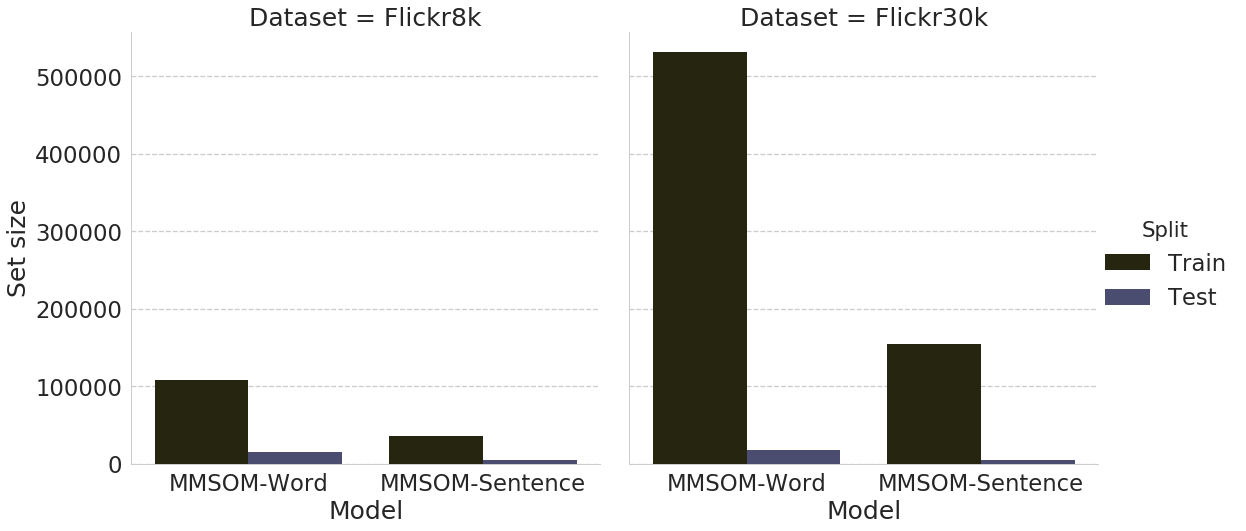
\includegraphics[width=\textwidth]{images/image_retrieval_data_info.png}
    \caption{Train and test sizes of the datasets used for the image retrieval experiments.}
    \label{fig:ImageRetrievalDatasetSizes}
\end{figure}

\begin{table}[h]
    \centering
    \begin{footnotesize}
        \begin{tabularx}{\textwidth}{|X|c|c|c|}
            \hline
            Model                           & Dataset  & Train set size & Test set size \\
            \hline
            \multirow{2}{*}{MMSOM-Word}     & Flikr8K  & 108,490        & 15,172         \\ 
            \cline{2-4}                     & Flikr30K & 530,682        & 17,391         \\ 
            \hline
            \multirow{2}{*}{MMSOM-Sentence} & Flikr8K  & \ \:35,416     & \ \:5000        \\
            \cline{2-4}                     & Flikr30K & 153,915        & \ \:5000        \\
            \hline
        \end{tabularx}
    \end{footnotesize}
    \caption{Train and test sizes of the datasets used for the image retrieval experiments.}
    \label{tab:ImageRetrievalDatasetSizes}
\end{table}

\begin{figure}[h]
    \centering
    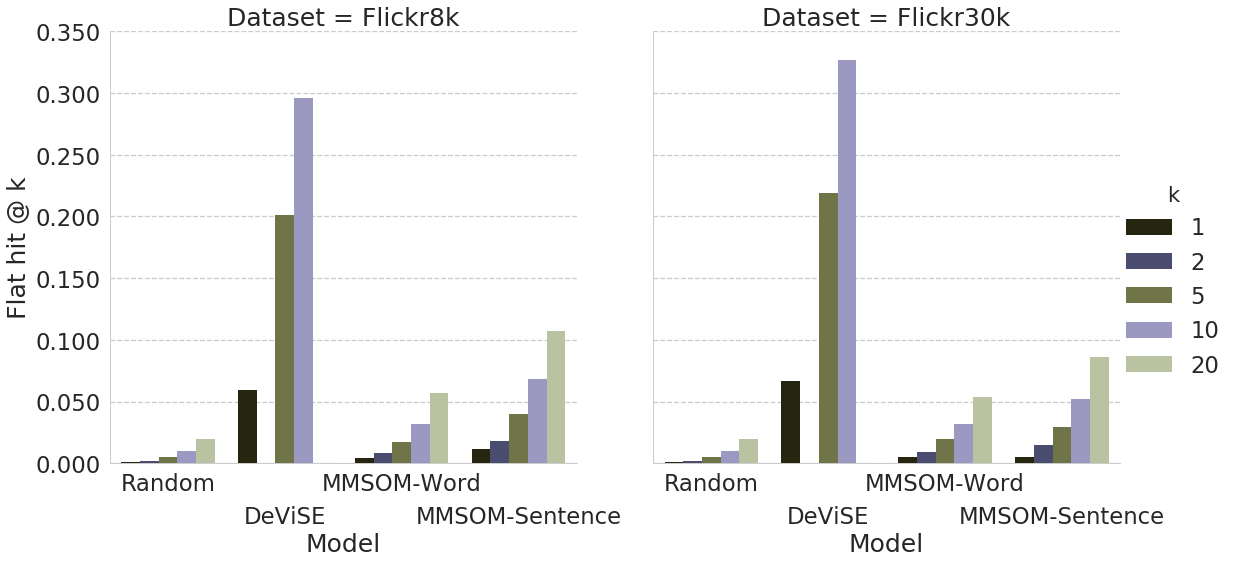
\includegraphics[width=\textwidth]{images/image_retrieval_results.png}
    \caption{Results for the image retrieval experiments. The results for the \texttt{DeViSE} model were reported in \cite{karpathy2014deep}.}
    \label{fig:ImageRetrievalResults}
\end{figure}

\begin{table}[h]
    \begin{footnotesize}
        \begin{tabularx}{\textwidth}{|X|c|c|c|c|c|c|}
            \hline
            \multirow{2}{*}{Model}          & \multirow{2}{*}{Dataset} & \multicolumn{5}{c|}{Flat hit @ $k$} \\
            \cline{3-7}                     &                          & 1      & 2      & 5      & 10     & 20     \\ 
            \hline
            \multirow{2}{*}{Random}         & Flickr8K                  & 0.0010 & 0.0020 & 0.0050 & 0.0100 & 0.0200 \\ 
            \cline{2-7}                     & Flickr30K                 & 0.0010 & 0.0020 & 0.0050 & 0.0100 & 0.0200 \\ 
            \hline
            \multirow{2}{*}{DeViSE}\cite{frome2013devise}
                                            & Flickr8K                  & \textbf{0.0590} & ------ & \textbf{0.2010} & \textbf{0.2960} & ------ \\ 
            \cline{2-7}                     & Flickr30K                 & \textbf{0.0670} & ------ & \textbf{0.2190} & \textbf{0.3270} & ------ \\ 
            \hline
            \multirow{2}{*}{MMSOM-Word}     & Flickr8K                  & 0.0040 & 0.0085 & 0.0173 & 0.0316 & 0.0566 \\ 
            \cline{2-7}                     & Flickr30K                 & 0.0055 & 0.0091 & 0.0194 & 0.0321 & 0.0536 \\ 
            \hline
            \multirow{2}{*}{MMSOM-Sentence} & Flickr8K                  & 0.0114 & 0.0180 & 0.0396 & 0.0680 & 0.1072 \\ 
            \cline{2-7}                     & Flickr30K                 & 0.0054 & 0.0146 & 0.0296 & 0.0518 & 0.0864 \\ 
            \hline
        \end{tabularx}
    \end{footnotesize}
    \caption{Results for the image retrieval experiments. The results for the \texttt{DeViSE} model were reported in \cite{karpathy2014deep}.}
    \label{tab:ImageRetrievalResults}
\end{table}

\subsection{Analysis and interpretation of results}\label{subsec:ImageRetrievalAnalysis}

The results clearly show that our approach was not appropriate for this task. One possible reason could lie in our training procedure. \Figref{Flickr30kWordFreq} shows the distribution of word frequencies for the Flickr30K dataset. As we can see, most of the words have a very low frequency, with a few having a relatively high frequency. Given the training procedure of the SOM, this could lead to the SOM-units corresponding to high frequency words converging correctly, while the SOM-units corresponding to low frequency words cannot converge.

\begin{figure}[h]
    \centering
    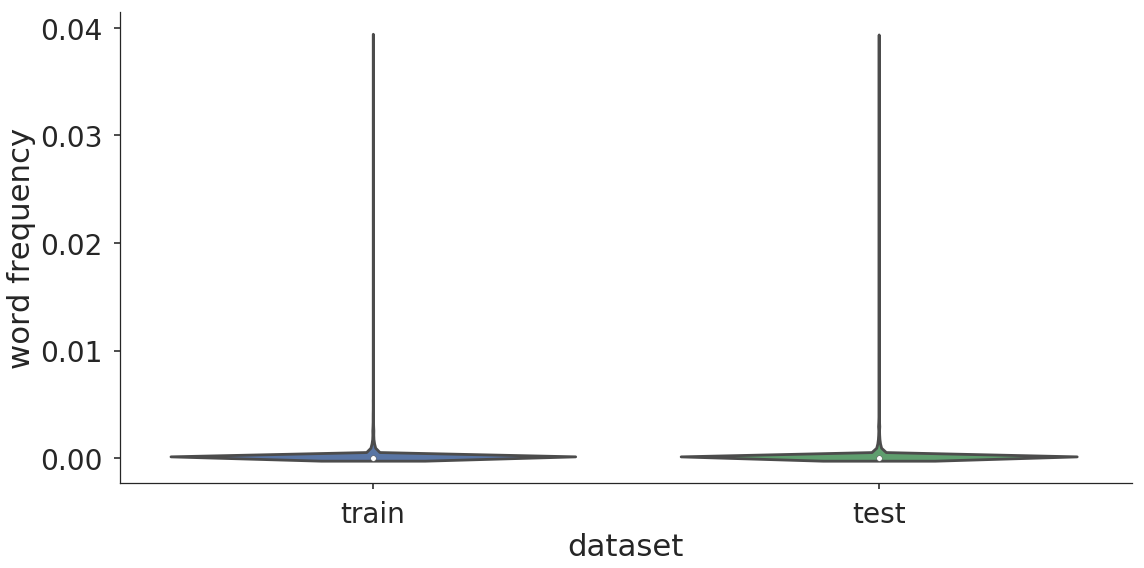
\includegraphics[width=\textwidth]{images/flickr30k_word_frequency.png}
    \caption{Word frequency distributions in the training and test datasets for Flickr30K, using the \texttt{MMSOM-Word} model. A higher word frequency means that the word was present in more sentences.}
    \label{fig:Flickr30kWordFreq}
\end{figure}

Possible solutions include augmenting the dataset to correct the imbalance, modifying the learning rate of the SOM training procedure according to the inverse of the word frequency, or using a completely different vector quantization method.

One more thing to take into account is the suitability of our performance measure. \Figref{ImageRetrievalStreetFail} shows some of the images retrieved for the query word "street" by the \verb|SOM-Sentence| model from the Flickr30K test set, with their descriptions at the top. As we can see, none of the descriptions contain the query word. Nonetheless, every scene takes place in a street setting. These cases would count as retrieval failures for the "flat hit @ $k$" measure, even though they seem to be correct. An alternative performance metric could be the "hierarchical hit @ k", explained in \secref{ZeroShotLearning}, \eqref{h_at_k}. The results for low values of $k$ are improved by using this metric, as shown in \tabref{ImageRetrievalHierarchical} for the \verb|MMSOM-Word| model on the Flickr8K dataset. A notion of why "hierarchical hit @ k" could be useful for image retrieval can be seen in \figref{ImageRetrievalSynsets}. The textual description of a retrieved image could contain any of the nodes in the graph, without containing the literal "street", and still be considered a relevant result for the query "street" by a human.
However, we have not found references of it being used in literature in this way, therefore its applicability in image retrieval is open to question.

\begin{figure}[h]
    \centering
    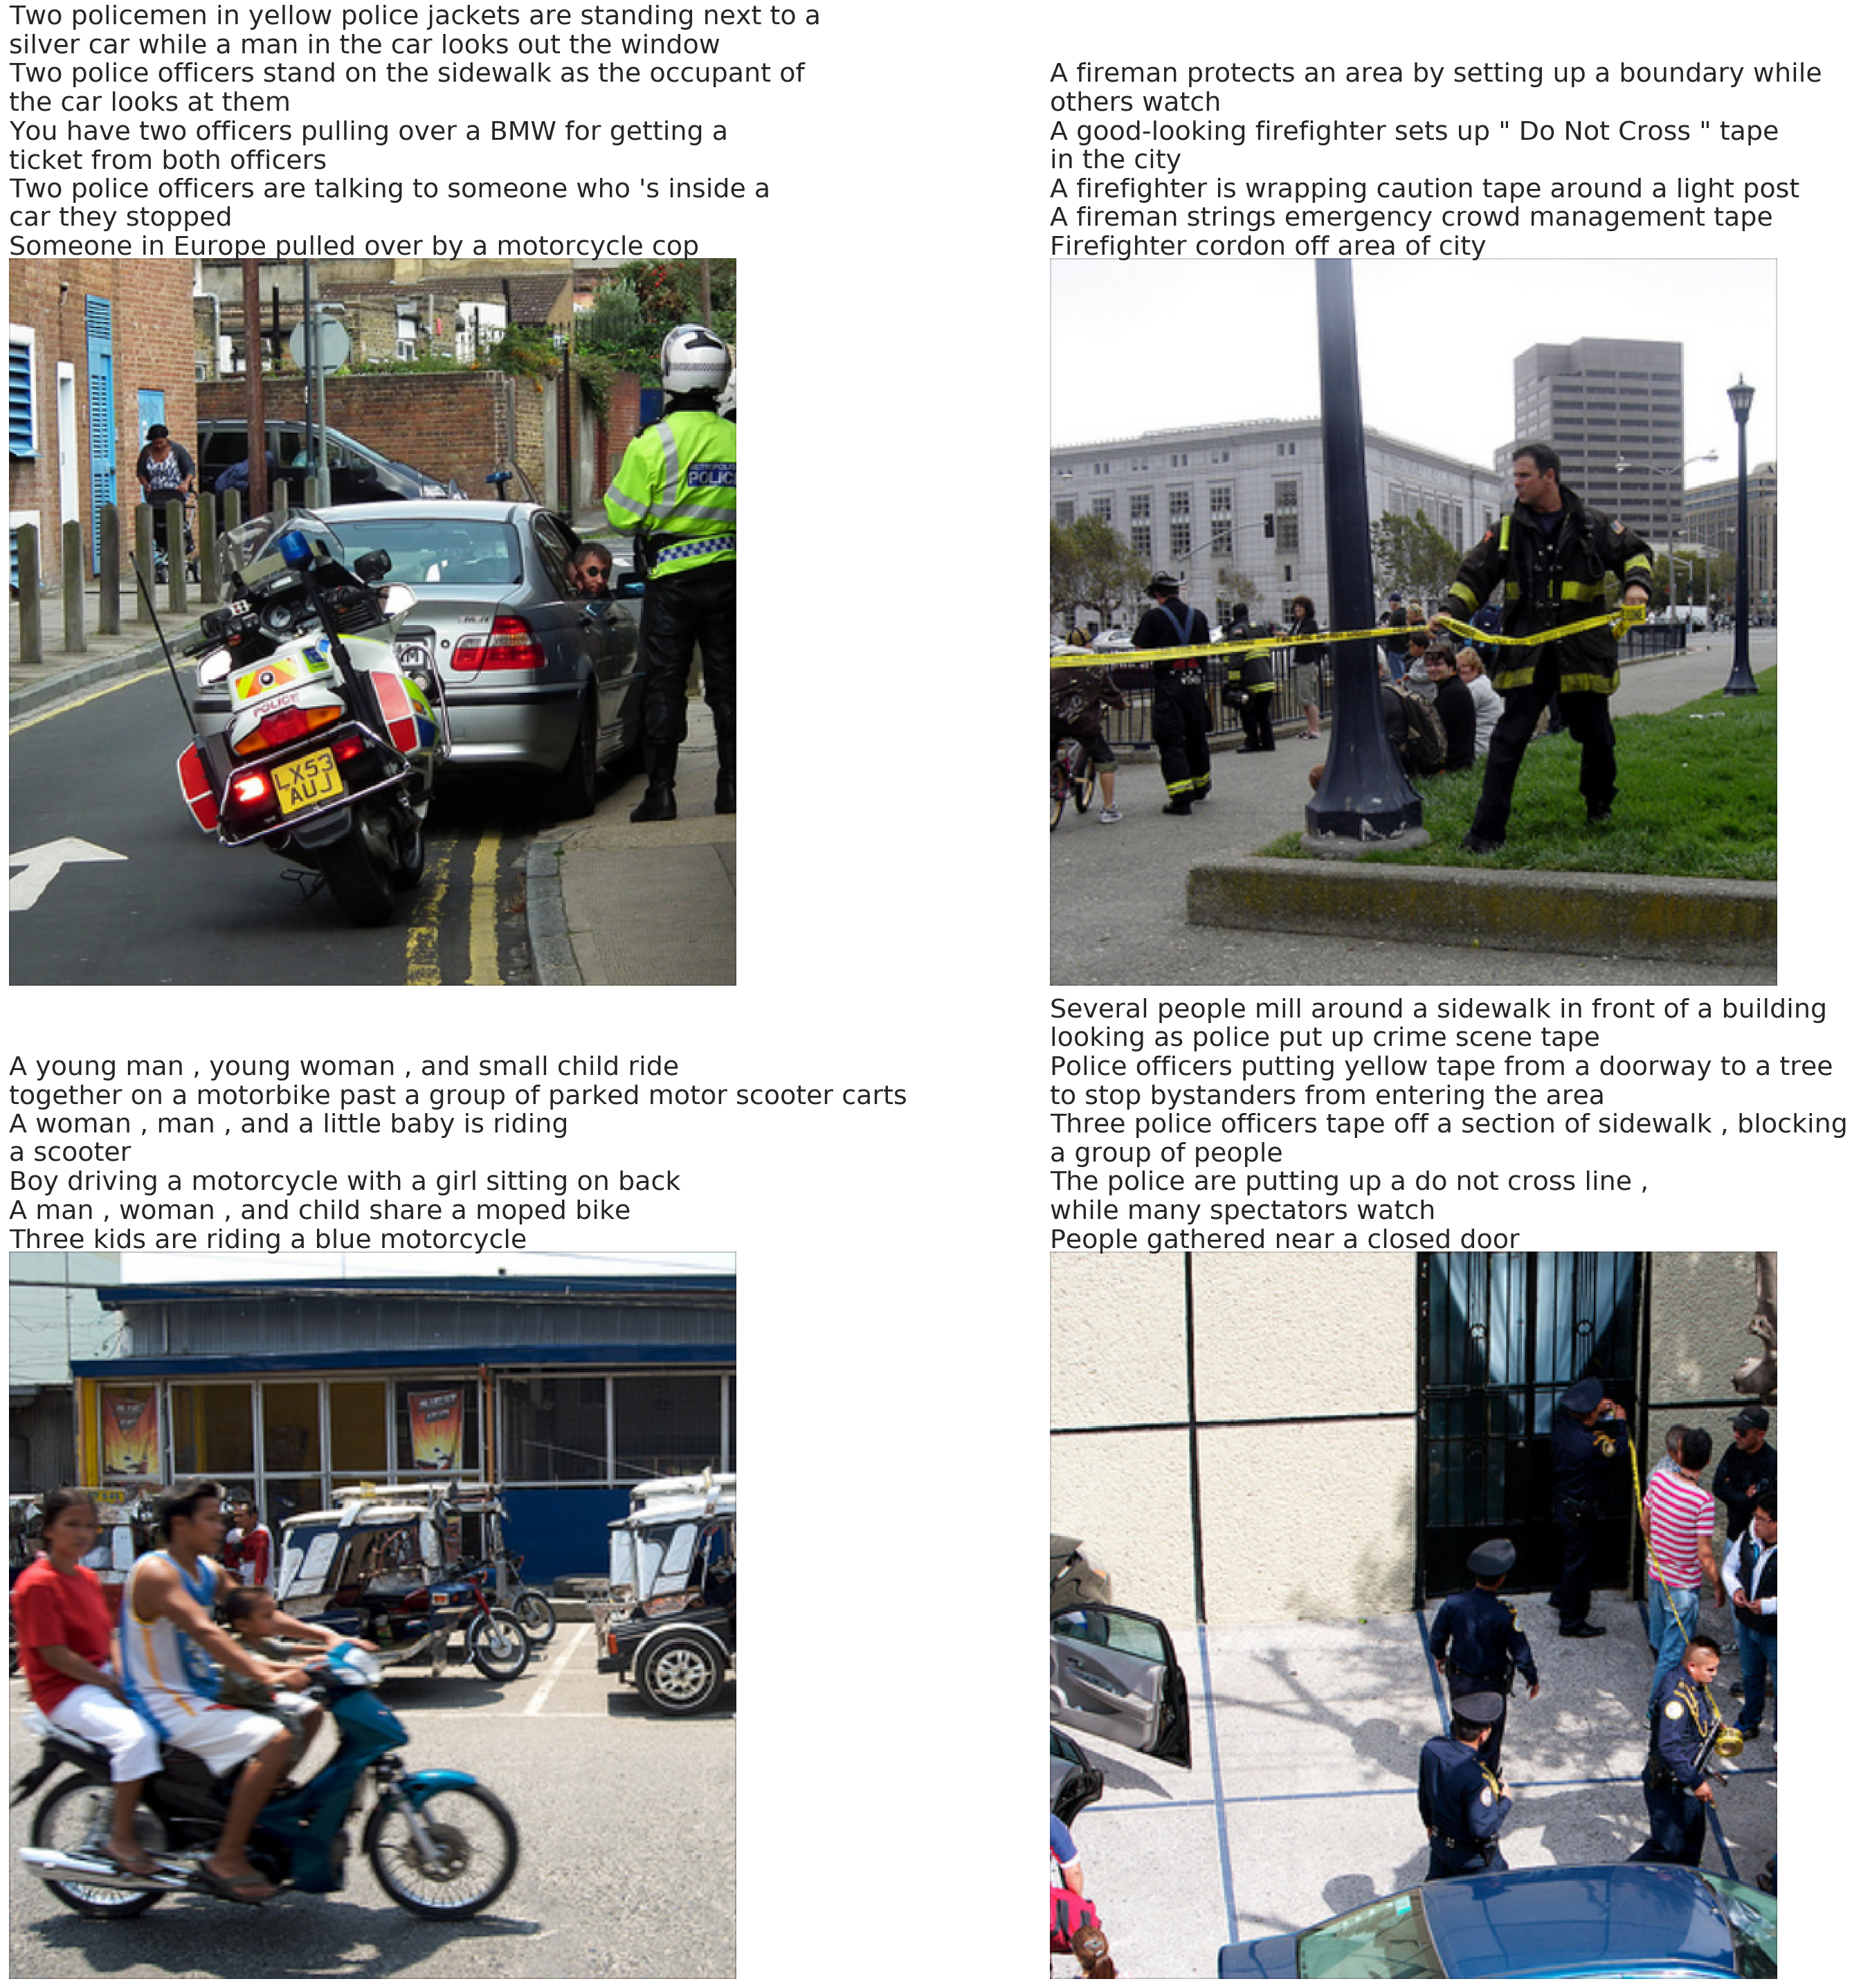
\includegraphics[width=\textwidth]{images/image_retrieval_street_fail.png}
    \caption{Images retrieved for the query word "street" by the \texttt{SOM-Sentence} model from the Flick30K test set}
    \label{fig:ImageRetrievalStreetFail}
\end{figure}

\begin{figure}[h]
    \centering
    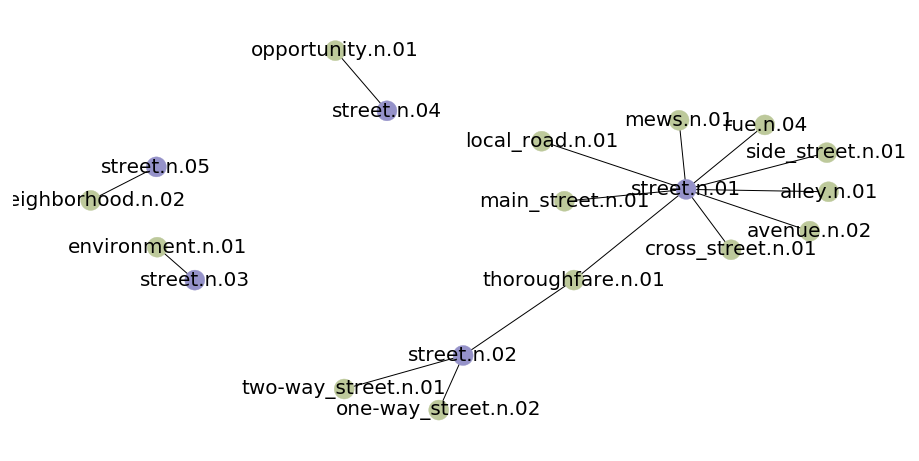
\includegraphics[width=\textwidth]{images/image_retrieval_fail_synsets.png}
    \caption{Hypernym-Hyponym closure (in orange) for the WordNet synsets corresponding to the word "street" (in green).}
    \label{fig:ImageRetrievalSynsets}
\end{figure}

\begin{table}[h]
    \begin{footnotesize}
        \begin{tabularx}{\textwidth}{|X|c|c|c|c|c|}
            \hline
            \multirow{2}{*}{Performance metric} & \multicolumn{5}{c|}{Flat hit @ $k$} \\
            \cline{2-5}                         & 1      & 2      & 5      & 10     & 20       \\ 
            \hline
            Flat hit @ k                        & 0.0040 & 0.0085 & 0.0173 & 0.0316 & 0.0566   \\ 
            \hline
            Hierarchical hit @ k                & N/A    & 0.0270 & 0.0282 & 0.0264 & 0.0189   \\ 
            \hline
        \end{tabularx}
    \end{footnotesize}
    \caption{Comparison of results using the "Flat hit @ k" vs "Hierarchical hit @ k" performance metrics for the \texttt{MMSOM-Word} model on the Flickr8K dataset.}
    \label{tab:ImageRetrievalHierarchical}
\end{table}

Given the sizes of the image embeddings relative to the word embeddings (4096 vs. 300) and our choice of distance metric, the images are going to have a \textasciitilde 13 times the weight of the words in any distance calculation. This effect could be offset by dividing each embedding by its length\footnote{$new\_img\_emb = img\_emb/4096; new\_wrd\_emb = wrd\_emb/300; $}, or by normalizing each embedding to unit euclidean norm before concatenation\footnote{$new\_img\_emb = img\_emb/\Vert img\_emb \Vert_2; new\_wrd\_emb = wrd\_emb/\Vert wrd\_emb \Vert_2; $}. We explored these alternatives using the \verb|MMSOM-Word| model on the Flickr8K dataset, but found that they provided worse results. We also tried to use the neighborhood relationships in the SOM by retrieving, for each of the k best matching units (BMUs) in the SOM, the single image in the test dataset nearest to that BMU\footnote{In of our final procedure we retrieved the k nearest images in the test dataset nearest to the the single BMU in the SOM}. This approach also provided worse results than our final procedure. The results of these failed alternatives are shown in \figref{ImageRetrievalFailed} and \tabref{ImageRetrievalFailed}. In light of this, we decided to avoid re-scaling the embeddings, normalizing them to unit lenght or using the SOM neighborhood in our final experiments.

\begin{figure}[h]
    \centering
    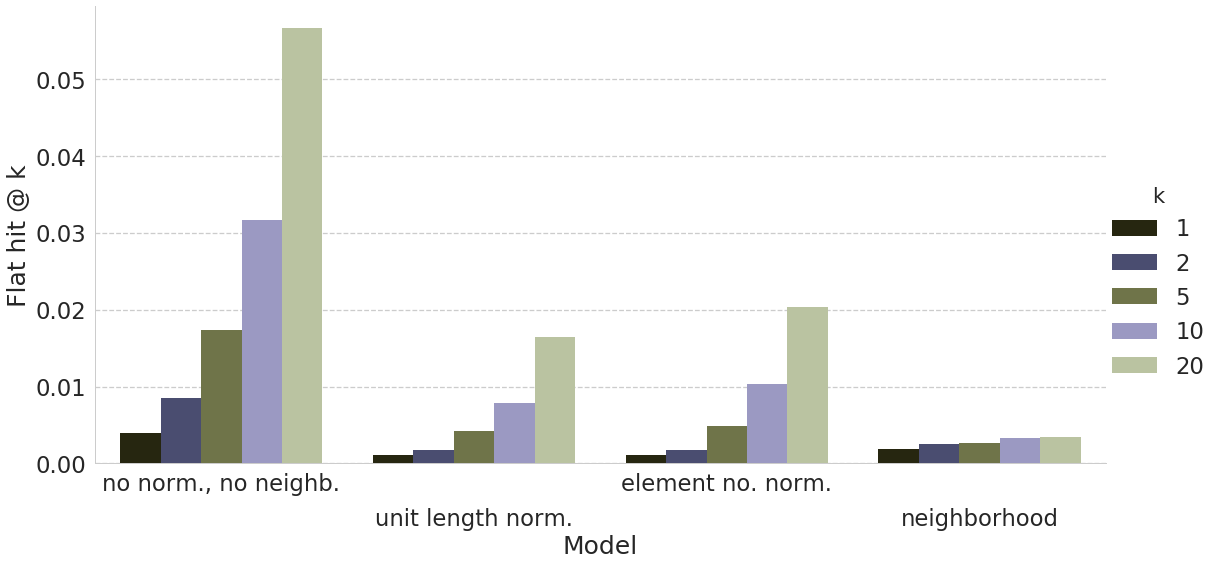
\includegraphics[width=\textwidth]{images/image_retrieval_fail_results.png}
    \caption{Results for the some failed approaches to the image retrieval experiments. \texttt{no norm, no neighb.}, \texttt{unit length norm.}, \texttt{element no. norm.} and \texttt{neighborhood} correspond, respectively, to \texttt{MMSOM-Word (no normalization, no neighborhood)}, \texttt{MMSOM-Word (unit length normalization)}, \texttt{MMSOM-Word (division by number of elements)} and \texttt{MMSOM-Word (neighborhood)} in \tabref{ImageRetrievalFailed}.}
    \label{fig:ImageRetrievalFailed}
\end{figure}

\begin{table}[h]
    \begin{footnotesize}
        \begin{tabularx}{\textwidth}{|X|c|c|c|c|c|}
            \hline
            \multirow{2}{*}{Model}                         & \multicolumn{5}{c|}{Flat hit @ $k$}        \\
            \cline{2-6}                                    & 1      & 2      & 5      & 10     & 20     \\ 
            \hline
            MMSOM-Word (no normalization, no neighborhood) & 0.0040 & 0.0085 & 0.0173 & 0.0316 & 0.0566 \\ 
            \hline
            MMSOM-Word (unit length normalization)         & 0.0011 & 0.0017 & 0.0042 & 0.0079 & 0.0165 \\ 
            \hline
            MMSOM-Word (division by number of elements)    & 0.0011 & 0.0018 & 0.0049 & 0.0103 & 0.0203 \\ 
            \hline
            MMSOM-Word (neighborhood)                      & 0.0019 & 0.0025 & 0.0027 & 0.0033 & 0.0034 \\ 
            \hline
        \end{tabularx}
    \end{footnotesize}
    \caption{Results for the some failed approaches to the image retrieval experiments. \texttt{MMSOM-Word (no normalization, no neighborhood)} is our final approach, shown in \tabref{ImageRetrievalResults}. \texttt{MMSOM-Word (unit length normalization)} normalizes the embedding of each modality to unit length individually. \texttt{MMSOM-Word (division by number of elements)} divides the image embedding by 4096 and the word embedding by 300. \texttt{MMSOM-Word (neighborhood)} retrieves, for each of the k BMUs in the SOM, the single image in the test dataset nearest to that BMU.}
    \label{tab:ImageRetrievalFailed}
\end{table}

\end{document}

\documentclass[a4paper]{standalone}

% use this declaration to set specific page margins
%\usepackage[a4paper , lmargin = {2.7cm} , rmargin = {2.9cm} , tmargin = {2.7cm} , bmargin = {4.6cm} ]{geometry}
\usepackage[a4paper]{geometry}
\usepackage[ngerman, english]{babel}

\usepackage[utf8]{inputenc}
\usepackage[boxed]{algorithm2e}
\usepackage{amsmath}
\usepackage{amssymb}
\usepackage{authblk}
\usepackage{caption}
\usepackage{cleveref}
\usepackage [autostyle, english = american]{csquotes}
\usepackage{fontenc}
\usepackage{fontspec}
\usepackage{graphicx}
\usepackage[pagebackref=true]{hyperref}
\usepackage{multirow}
\usepackage[section]{placeins}
\usepackage{refstyle}
\usepackage{standalone}
\usepackage{subcaption}
\usepackage{tabularx}
\usepackage{url}
\usepackage{scrpage2}					% header and footer line


% header and footer line - no header & footer line on pages where a new chapter starts
\pagestyle{scrheadings}
\ohead{Mixing Text and Image Modalities in Artificial Neural Networks}
\ihead{Mario Tambos}
\ofoot[]{\thepage}
\ifoot{Master's Thesis, Mario Tambos, TU Berlin, Fachgebiet NI, 2018}

\MakeOuterQuote{"}

\newref{part}{name=part~,Name=Part~,names=parts~,Names=Parts~}
\newref{alg}{name=algorithm~,Name=Algorithm~,names=algorithms~,Names=Algorithms~}
\newref{sec}{name=section~,Name=Section~,names=sections~,Names=Sections~}
\newref{subsec}{name=subsection~,Name=Subsection~,names=subsections~,Names=Subsections~}

\newcommand{\vect}[1]{\mathbf{#1}}

\newcommand{\vecx}{\vect{x}}
\newcommand{\Dcal}{\mathcal{D}}
\newcommand{\Sbf}{\Sigma}
\newcommand{\Sbfs}{\Sigma^\star}
\newcommand{\Rbb}{\mathbb{R}}
\newcommand{\Nbb}{\mathbb{N}}

\makeatletter
\setlength{\@fptop}{0pt}
\makeatother

\makeatletter
\AtBeginDocument{%
    \expandafter\renewcommand\expandafter\subsection\expandafter{%
        \expandafter\@fb@secFB\subsection
    }%
}
\makeatother


\begin{document}
\section{Image Classification}\label{sec:ImageClassification}

In this section we explore the performance of our model on the ImageNet Large Scale Visual Recognition Challenge 2012 (ILSVRC2012). This task consists of a classification problem, where we are trying to predict the class of an image, based solely on its pixel values. For this we use the ILSVRC2012 1k dataset, consisting of 1,281,167 train and 50,000 test images, divided into 1000 different object classes.

\begin{figure}[h]
    \centering
    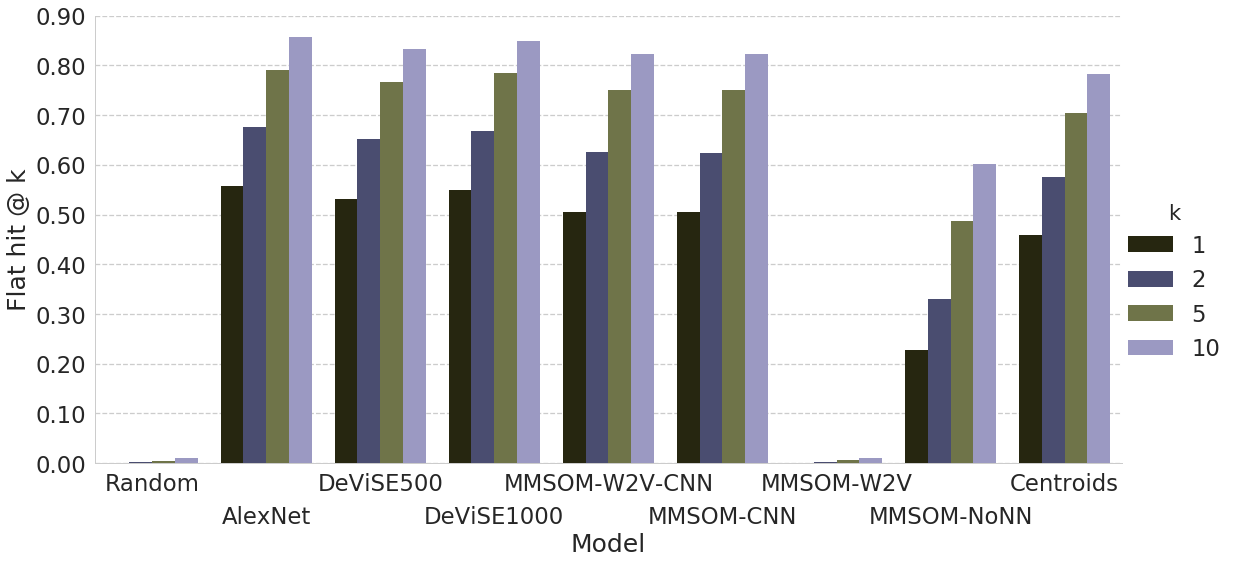
\includegraphics[width=\textwidth]{images/image_classification_results.png}
    \caption{ImageNet 1K Image classification experiment}
    \label{fig:ImageNet1KResults}
\end{figure}


\begin{table}[h]
    \begin{footnotesize}
        \begin{tabularx}{\textwidth}{|X|c|c|c|c|}
            \hline
            \multirow{2}{*}{Model} & \multicolumn{4}{ c|}{Flat hit @ $k$} \\
            \cline{2-5}            & 1               & 2               & 5               & 10        \\
            \hline
            Random guess           & 0.0010          & 0.0020          & 0.0050          & 0.0100    \\
            AlexNet\cite{krizhevsky2012imagenet}
                                   & \textbf{0.5565} & \textbf{0.6755} & \textbf{0.7906} & \textbf{0.8563}    \\
            DeViSE500\cite{frome2013devise}
                                   & 0.5320          & 0.6520          & 0.7670          & 0.8330    \\
            DeViSE1000\cite{frome2013devise}
                                   & 0.5490          & 0.6690          & 0.7840          & 0.8500    \\
            \hline
            MMSOM-W2V-CNN          & 0.5058          & 0.6249          & 0.7508          & 0.8233    \\
            MMSOM-CNN              & 0.5057          & 0.6247          & 0.7505          & 0.8234    \\
            MMSOM-W2V              & 0.0010          & 0.0020          & 0.0058          & 0.0111    \\
            MMSOM-NoNN             & 0.2279          & 0.3304          & 0.4867          & 0.6026    \\
            Centroids              & 0.4585          & 0.5764          & 0.7033          & 0.7821    \\
            \hline
        \end{tabularx}
    \end{footnotesize}
    \caption{ImageNet 1K Image classification experiment}
    \label{tab:ImageNet1KResults}
\end{table}

The results of our experiments for this section are presented in \figref{ImageNet1KResults}, and also in \tabref{ImageNet1KResults}, for a detailed reference. The models \verb|MMSOM-W2V-CNN|, \verb|MMSOM-CNN| and \verb|MMSOM-W2V| were trained and evaluated as described in \algref{TrainImgNetSOM, RetrieveImgNetLabel}. A schematic view of the network architecture used is shown in \figref{ImageNetExperimentArchitecture}. The \verb|Classifier| in the figure is a simple 3-layer, fully connected feed-forward NN, with 4396 input neurons, 4396 hidden neurons and 1000 output neurons. The reason for choosing this particular architecture was to introduce a non-linearity between the multi-modal embedding and the \verb|Softmax| layer in the \verb|Classifier|. Due to time constraints, we performed no hyper-parameter exploration.

Among \verb|MMSOM-W2V-CNN|, \verb|MMSOM-W2V| and \verb|MMSOM-CNN|, only \verb|MMSOM-W2V-CNN| was trained, whereas at test time:
\begin{itemize}
    \item \verb|MMSOM-CNN| has the input neurons corresponding to the GloVe embedding (green in the figure) in its classifier neural network zeroed out.
    \item \verb|MMSOM-W2V| has the input neurons corresponding to the image embedding (blue in the figure) in its classifier neural network zeroed out.
    \item \verb|MMSOM-W2V-CNN| works with both the image and GloVe embeddings.
\end{itemize}

\begin{figure}[h]
    \centering
    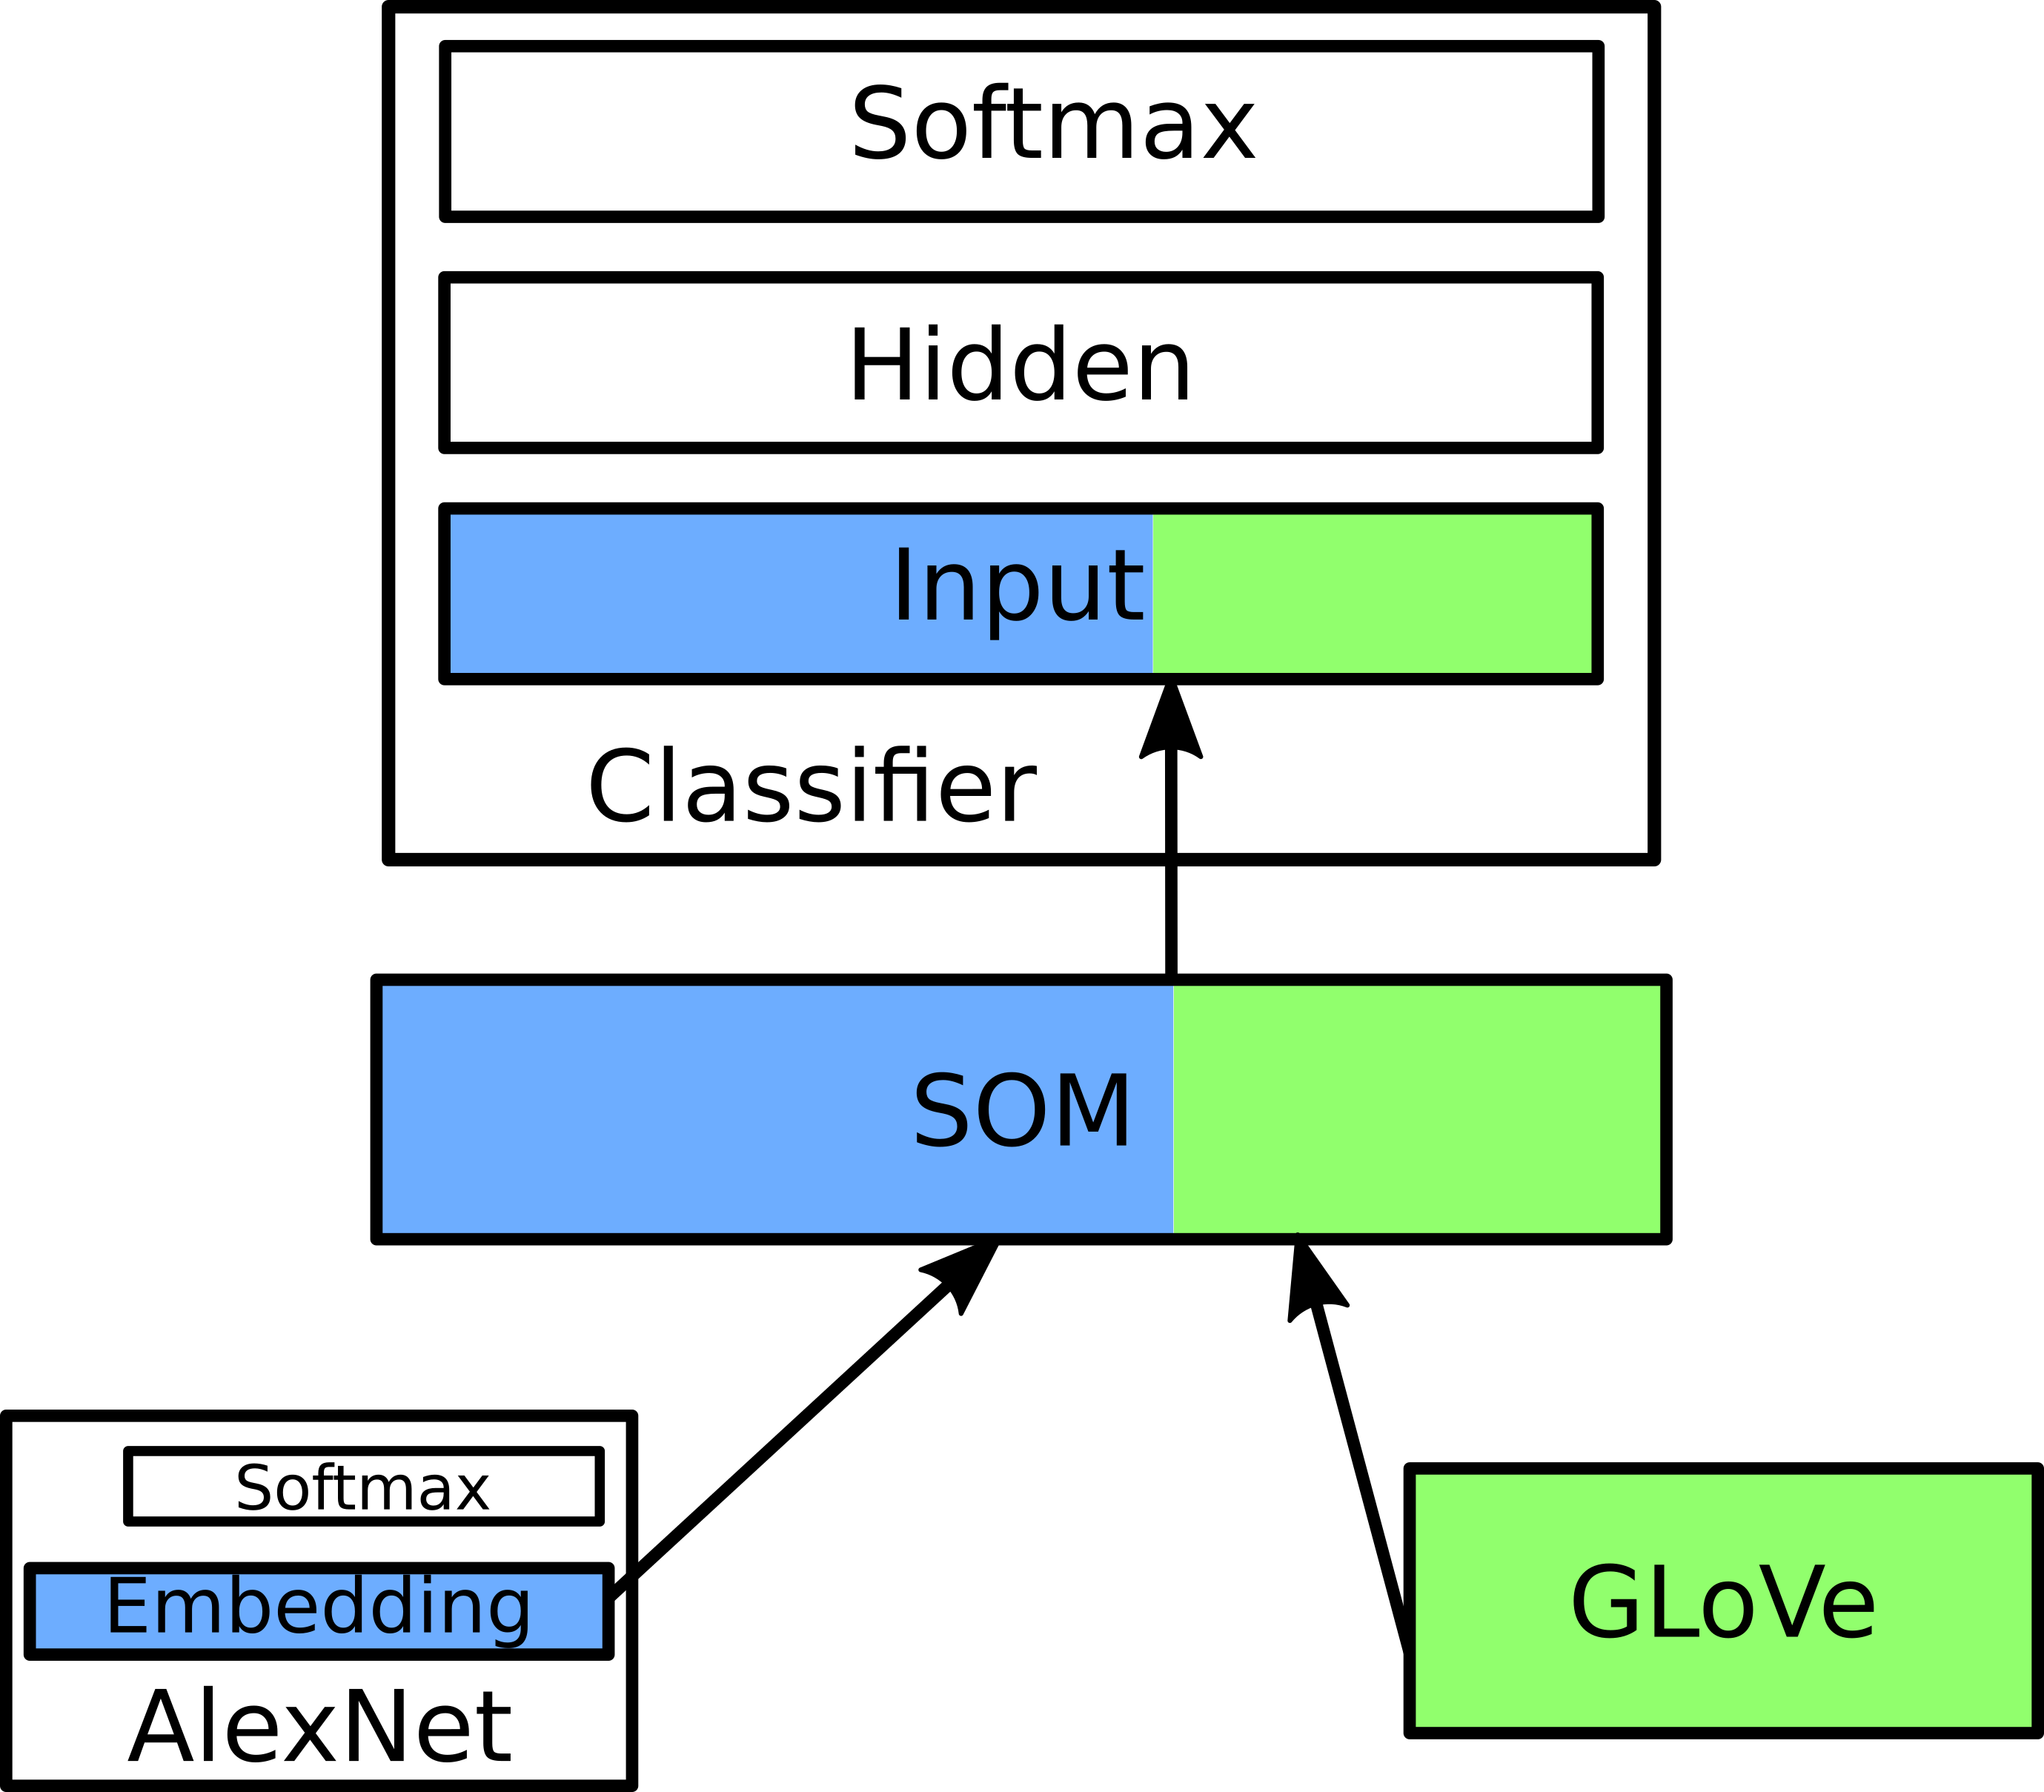
\includegraphics[width=0.5\textwidth]{images/ImageNetExperimentArchitecture.png}
    \caption{Network architecture for the Image classification Experiment. All layers in the Alex net model were used, except for the softmax layer. Blue indicates An image embedding, green indicates a word embedding.}\label{fig:ImageNetExperimentArchitecture}
\end{figure}

In contrast, \verb|MMSOM-NoNN| uses no classifier neural network. It relies instead on \algref{RetrieveWord}, with the 1000 object classes as its word search space, i.e., the \verb|w2vModel| contains in its vocabulary only the 1000 words corresponding to the object classes.

Finally, \verb|Centroids| uses neither SOM model nor classifier neural network. Its training consists on calculating and storing the mean image embedding for each object class in the training set; these form 1000 centroids. At test time, for each test image the nearest centroid to the test image is calculated, and the prediction is the label corresponding to that centroid. The method is explained in detail in \algref{RetrieveCentroidLabel}.

\begin{algorithm}[ht]
    \SetKwFunction{RetrieveCentroidLabel}{RetrieveImgNetLabel}
    \RetrieveCentroidLabel{$\Dcal_N$, $\vecx$}\\
    \KwData{
        $\Dcal_N = \{(\vecx_i, w_i); \vecx_i \in \Rbb^{M_1, M_2, 3}, w_i \in \Sbfs, i \in \Nbb_{\leq N}\}$: Dataset of image-word pairs. In this case, $\Sbfs$ consist of 1000 different words (training labels).\\
        $\vecx \in \Rbb^{M_1, M_2, 3}$: Image we want to retrieve an associated ImageNet label for.
    }
    \KwResult{$l_w \in \Rbb^{1000}$: encoded label associated with $\vecx$}
    \Begin{
        $\mathbf{cnnModel} \gets$ Load pre-trained AlexNet model.\;
        $centroids \gets (\Rbb^{1000\times 4096}, \Rbb^{1000})$\;
        \For{$w_i\ \mathbf{in}\ \Sbfs$}{
            $centroids[i, 0] \gets \mathbf{mean}(\{\mathbf{cnnModel.project}(\vecx_j): (\vecx_j, w_j) \in \Dcal_N \wedge w_j=w_i\})$\;
            $centroids[i, 1] \gets \mathbf{encodeLabel}(w_i)$\;
        }
        $cnnProj \gets \mathbf{cnnModel.project}(\vecx)$\;
        $nearestCentr \gets \arg \min_{c \in centroids} \Vert cnnProj - c[0] \Vert^2$\;
        $l_w \gets nearestCentr[1]$
    }
    \caption{Label prediction procedure for the ImageNet1K classification task using the \texttt{Centroids} approach.}\label{alg:RetrieveCentroidLabel}
\end{algorithm}

\subsection{Notes on \texttt{MMSOM-W2V-CNN} training}

Since we are dealing with 1000 words (object classes), we decided to use a square grid of $32\times 32 = 1024$ units for the SOM model. We hoped that, after training, at least one SOM unit would be associated with an object class. The SOM model was trained for 40 epochs, whereas the top NN model was trained for 100 epochs. These settings seemed sufficient for the NN classifier to converge to a minimum, therefore, we avoided optimizing the number of training epochs.

Several optimization methods were tried for the training of the \verb|Classifier| NN in \verb|MMSOM-W2V-CNN|: from plain stochastic gradient descent (SGD) to state-of-the-art approaches like Adam \cite{kingma2014adam}. Sadly, all adaptive methods failed to converge, being unable to improve on \textasciitilde 0.4 "flat hit @ 5" accuracy on the validation set. This is perhaps related to the work of Wilson et al. \cite{Wilson2017}. Therefore, we used plain SGD to train our final model.

We decided to use L1-regularization on the input layer and L2-regularization on the hidden layer. The idea was to analyze the relevance of the different embedding components on the classification. By using L1-regularization we aimed to induce sparsity in the input weights. Then, if the norm of a weight vector for a given input neuron is close to zero, this would mean that the input neuron was irrelevant to improving the accuracy of the model during training.

\subsection{Analysis and interpretation of results}\label{subsec:ImageClassificationAnalysis}

Although the performance of \verb|MMSOM-W2V-CNN| was lower than the DeViSE and AlexNet approaches, \verb|MMSOM-W2V-CNN| was close to them. This indicates that \verb|MMSOM-W2V-CNN| could be improved by a better training procedure (data augmentation, better optimization settings, etc.), or by alterations in the architecture. However, the extremely low impact of the GloVE embeddings on the training casts a doubt on whether the proposed approach was indeed useful. We expected the \verb|w2vModel| to provide extra information to the \verb|Classifier| NN, which was clearly not the case in practice.

Regarding the effects of the L1-regularization, from the 4096 input weight vectors for the CNN embedding in \verb|MMSOM-W2V-CNN|, 2056 had an euclidean norm lower than $10E^{-4}$ (~50\% of the vectors). In contrast, from the 300 input weight vectors for the GloVe embedding, 297 had an euclidean norm lower than $10E^{-4}$ (~99\% of the vectors). In other words, the GloVe embeddings had close to no influence on the training procedure. This concurs with the results from \tabref{ImageNet1KResults} for the \verb|MMSOM-W2V-CNN|, \verb|MMSOM-CNN| and \verb|MMSOM-CNN| models.

In contrast, \verb|MMSOM-NoNN| could present a better line of research. Even though it was behind both AlexNet and DeViSE, it was also far above the random guess baseline.

The \verb|Centroids| results gave us pause. They seem to imply that the images are clustered at the level of the CNN embedding, with each cluster corresponding to one ImageNet label, and with little overlap between clusters.
\end{document}

\documentclass[a4paper]{standalone}

% use this declaration to set specific page margins
%\usepackage[a4paper , lmargin = {2.7cm} , rmargin = {2.9cm} , tmargin = {2.7cm} , bmargin = {4.6cm} ]{geometry}
\usepackage[a4paper]{geometry}
\usepackage[ngerman, english]{babel}

\usepackage[utf8]{inputenc}
\usepackage[boxed]{algorithm2e}
\usepackage{amsmath}
\usepackage{amssymb}
\usepackage{authblk}
\usepackage{caption}
\usepackage{cleveref}
\usepackage [autostyle, english = american]{csquotes}
\usepackage{fontenc}
\usepackage{fontspec}
\usepackage{graphicx}
\usepackage[pagebackref=true]{hyperref}
\usepackage{multirow}
\usepackage[section]{placeins}
\usepackage{refstyle}
\usepackage{standalone}
\usepackage{subcaption}
\usepackage{tabularx}
\usepackage{url}
\usepackage{scrpage2}					% header and footer line


% header and footer line - no header & footer line on pages where a new chapter starts
\pagestyle{scrheadings}
\ohead{Mixing Text and Image Modalities in Artificial Neural Networks}
\ihead{Mario Tambos}
\ofoot[]{\thepage}
\ifoot{Master's Thesis, Mario Tambos, TU Berlin, Fachgebiet NI, 2018}

\MakeOuterQuote{"}

\newref{part}{name=part~,Name=Part~,names=parts~,Names=Parts~}
\newref{alg}{name=algorithm~,Name=Algorithm~,names=algorithms~,Names=Algorithms~}
\newref{sec}{name=section~,Name=Section~,names=sections~,Names=Sections~}
\newref{subsec}{name=subsection~,Name=Subsection~,names=subsections~,Names=Subsections~}

\newcommand{\vect}[1]{\mathbf{#1}}

\newcommand{\vecx}{\vect{x}}
\newcommand{\Dcal}{\mathcal{D}}
\newcommand{\Sbf}{\Sigma}
\newcommand{\Sbfs}{\Sigma^\star}
\newcommand{\Rbb}{\mathbb{R}}
\newcommand{\Nbb}{\mathbb{N}}

\makeatletter
\setlength{\@fptop}{0pt}
\makeatother

\makeatletter
\AtBeginDocument{%
    \expandafter\renewcommand\expandafter\subsection\expandafter{%
        \expandafter\@fb@secFB\subsection
    }%
}
\makeatother


\begin{document}
\section{Zero-shot learning}\label{sec:ZeroShotLearning}

In this final experiment we evaluate the performance of our method on a zero-shot learning task. Given a training set $\mathcal{D}^{(trn)}_N=\{(\vecx_i, y_i): \vecx_i \in \mathbf{X}, y_i \in \mathbf{Y}\}$ of N training pairs $(\vecx_i, y_i)$ and a model $\mathcal{M}$ trained on $\mathcal{D}^{(trn)}_N$, we want to evaluate $\mathcal{M}$ on a test dataset $\mathcal{D}^{(tst)}_M=\{(\vecx_j, \hat{y}_j): \vecx_j \in \mathbf{X}, \hat{y}_j \in \hat{\mathbf{Y}}\}$ of M test pairs $(\vecx_j, \hat{y}_j)$ with $\mathbf{Y} \neq \hat{\mathbf{Y}}$. It could be the case that $\mathbf{Y} \subsetneq \hat{\mathbf{Y}}$ or even $\mathbf{Y} \cap \hat{\mathbf{Y}} = \emptyset$.

In order to perform this experiment, and following Frome et al. \cite{frome2013devise}, we used three different datasets:
\begin{itemize}
%    \item ImageNet1K \cite{ILSVRC15}: is the dataset used in \secref{ImageClassification}.
    \item ImageNet21K \cite{ILSVRC15}: consists of 14,197,087 images divided into 21,841 different object classes.
    \item ImageNet1K - 2 Hops: was built by all images and classes in ImageNet21K, whose classes were at most 2 hops away in the WordNet \cite{miller1998wordnet} hierarchy from a class in ImageNet1K, the dataset used in \secref{ImageClassification}.
    \item ImageNet1K - 3 Hops: was built by all images and classes in ImageNet21K, whose classes were at most 3 hops away in the WordNet  hierarchy from a class in ImageNet1K.
\end{itemize}

Also like Frome et al. \cite{frome2013devise}, we used both the "flat hit @ k" employed \secref{ImageClassification}, as well as their "hierarchical hit @ k", defined as:

\begin{small}
    $$
        hierarchical\ hit @ k = \frac{1}{N}\sum_{N}^{i=1}\frac{\text{\# of model's top } k \text{ predictions} \in CorrectSet(trueLabel_i)}{k}\label{eq:h_at_k}\qquad (4.3)
    $$
\end{small}

where $CorrectSet(trueLabel_i)$ is created for each label in a test dataset as shown in \algref{CreateCorrectSet}, and $trueLabel_i$ is the true label corresponding to the $i$th image.
By reporting "hierarchical hit @ k" we try to take into account semantic similarities among the class labels: synonymy, hypernymy ("canine" is a hypernym of "dog"), coordinate terms ("wolf" is a coordinate term of "dog", and vice-versa), etc. Then, if our model predicted "pen" for an image with true label "pencil", "flat hit @ k" would be 0, but there is some $CorrectSet$ for which "hierarchical hit @ k" will be non-zero.

\begin{algorithm}[h]
    \SetKwFunction{CreateCorrectSet}{CreateCorrectSet}
    \CreateCorrectSet{$trueLabel$, $k$, $validLabels$}\\
    \KwData{
        
        $trueLabel$: class label in a test dataset.\\
        $k$: Minimum size of the $CorrectSet$.\\
        $validLabels$: set of labels allowed as members of $CorrectSet$.
    }
    \KwResult{$CorrectSet(trueLabel)$: equivalence set of labels for $trueLabel$}
    \Begin{
        $R \gets 0$\;
        \While{$|CorrectSet| < k$}{
            $radiusSet \gets $ all members of $validLabels$ that are $R$ hops from $trueLabel$ in the WordNet hierarchy.\;
            $CorrectSet \gets CorrectSet \cup radiusSet$\;
            $R \gets R + 1$\;
        }
    }
    \caption{$CorrectSet$ creation procedure, defined in \cite{frome2013devise}}\label{alg:CreateCorrectSet}
\end{algorithm}


The number of unique classes in the test datasets used for the zero-shot experiments, together with the mean sizes of the corresponding $CorrectSet$s at $k$, are shown in \figref{ZeroShotDatasetClassesNr} and \tabref{ZeroShotDatasetClassesNr}. In some cases, these numbers are extremely different from the ones reported by Frome et al.. Consequently, we decided not to include their results for comparison, as the methods we used for creating our test sets and calculating our performance metrics might not be comparable with theirs. Instead, we decided to use a random classifier as a baseline.

\begin{figure}[ht]
    \centering
    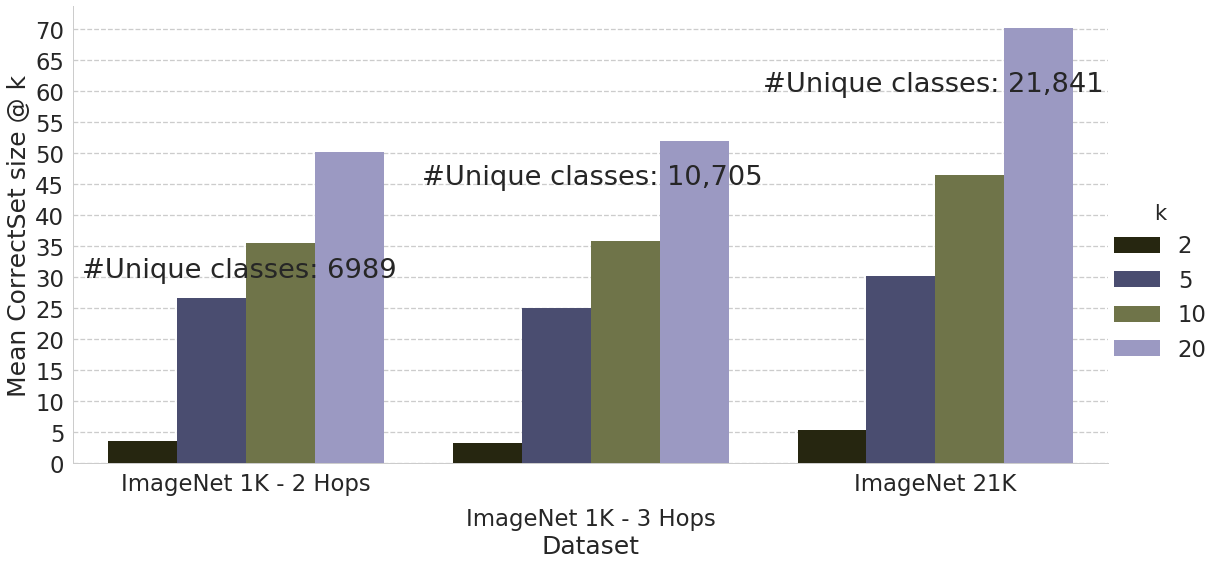
\includegraphics[width=\textwidth]{images/zero_shot_data_info.png}
    \caption{Number of unique classes in the test datasets used for the zero-shot experiments, together with the mean sizes of the corresponding $CorrectSet$s at $k$.}
    \label{fig:ZeroShotDatasetClassesNr}
\end{figure}

\begin{table}[h]
    \centering
    \begin{footnotesize}
        \begin{tabularx}{\textwidth}{|X|c|c|c|c|c|}
            \hline
            \multirow{2}{*}{Dataset} & \multirow{2}{*}{\# Unique classes} & \multicolumn{4}{c|}{Mean $CorrectSet$ size @ k} \\
            \cline{3-6}              &                                    & k=2      & k=5      & k=10     & k=20           \\ 
            \hline
%            ImageNet1K               & 1000                               & 3.062    & 16.031   & 25.413   & 41.583         \\ 
            ImageNet1K - 2 Hops      & 6989                               & 3.587    & 26.586   & 35.472   & 50.122         \\ 
            ImageNet1K - 3 Hops      & 10,705                             & 3.320    & 24.992   & 35.824   & 52.001         \\ 
            ImageNet21K              & 21,841                             & 5.350    & 30.160   & 46.517   & 70.111         \\ 
            \hline
        \end{tabularx}
    \end{footnotesize}
    \caption{Number of unique classes in the test datasets used for the zero-shot experiments, together with the mean sizes of the corresponding $CorrectSet$s at $k$.}
    \label{tab:ZeroShotDatasetClassesNr}
\end{table}


To execute the experiments in this section we employed the same \verb|MMSOM-W2V-CNN| model trained in \secref{ImageClassification}. However, in this case we did not work with the NN Classifier built into \verb|MMSOM-W2V-CNN|, but rather operated directly with the internal SOM model. Our predictions rely entirely on \algref{RetrieveWord}. The results we have obtained are shown in \tabref{ZeroShotFlatResults, ZeroShotHierarchicalResults} for the "flat hit @ k" and "hierarchical hit @ k" metrics, respectively.

\begin{figure}[h]
    \centering
    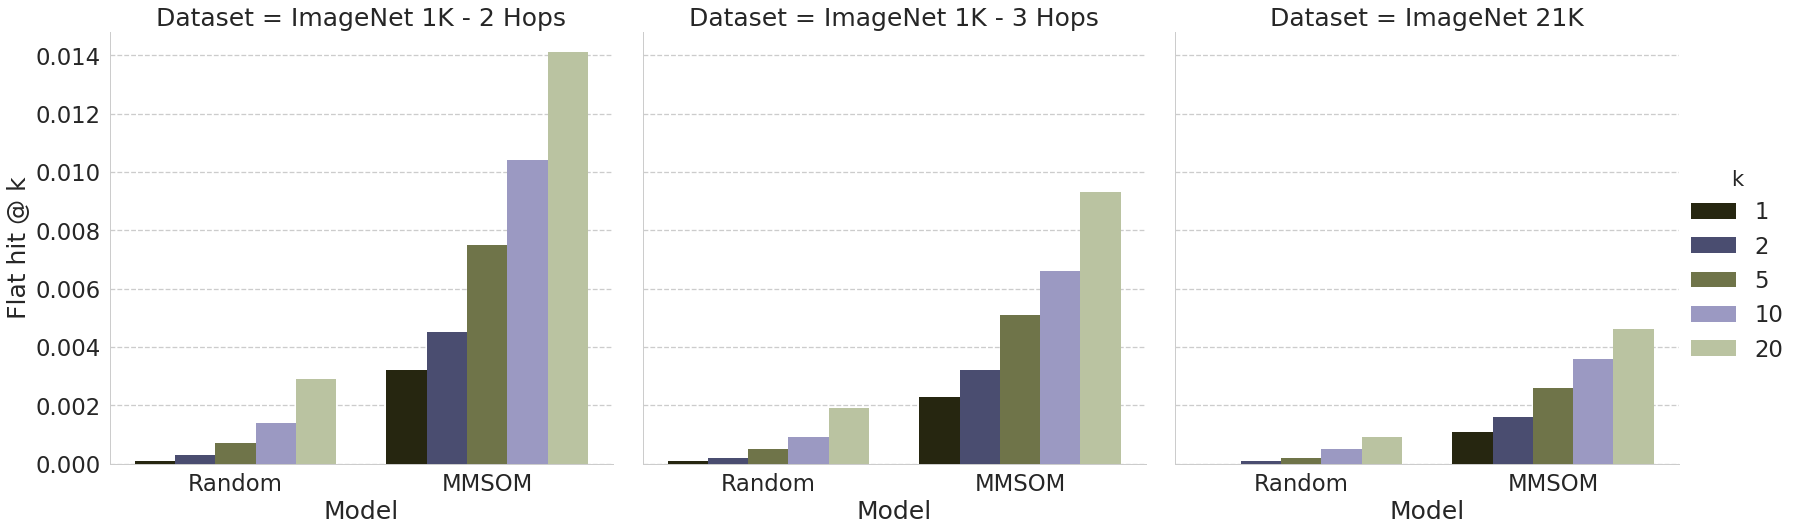
\includegraphics[width=\textwidth]{images/zero_shot_flat_results.png}
    \caption{Zero-shot learning experiment - "flat hit @ k" metric.}
    \label{figZeroShotFlatResults}
\end{figure}

\begin{table}[h]
    \centering
    \begin{footnotesize}
        \begin{tabularx}{\textwidth}{|X|c|c|c|c|c|c|}
            \hline
            \multirow{2}{*}{Dataset} & \multirow{2}{*}{Model}    & \multicolumn{5}{c|}{Flat hit @ $k$}        \\
            \cline{3-7}              &                           & 1      & 2      & 5      & 10     & 20     \\ 
%            \hline
%            \hline
%            \multirow{2}{*}{ImageNet1K}          & Random        & 0.0010 & 0.0020 & 0.0050 & 0.0100 & 0.0200 \\ 
%            \cline{2-7}                          & MMSOM         & 0.0241 & 0.0344 & 0.0515 & 0.0619 & 0.0790 \\ 
            \hline
            \hline
            \multirow{2}{*}{ImageNet1K - 2 Hops} & Random        & 0.0001 & 0.0003 & 0.0007 & 0.0014 & 0.0029 \\ 
            \cline{2-7}                          & MMSOM         & 0.0032 & 0.0045 & 0.0075 & 0.0104 & 0.0141 \\ 
            \hline
            \hline
            \multirow{2}{*}{ImageNet1K - 3 Hops} & Random        & $9.3414E^{-5}$ & 0.0002 & 0.0005 & 0.0009 & 0.0019 \\ 
            \cline{2-7}                          & MMSOM         & 0.0023         & 0.0032 & 0.0051 & 0.0066 & 0.0093 \\ 
            \hline
            \hline
            \multirow{2}{*}{ImageNet21K}         & Random        & $4.5785E^{-5}$ & $9.1571E^{-5}$ & 0.0002 & 0.0005 & 0.0009 \\ 
            \cline{2-7}                          & MMSOM         & 0.0011         & 0.0016         & 0.0026 & 0.0036 & 0.0046 \\ 
            \hline
        \end{tabularx}
    \end{footnotesize}
    \caption{Zero-shot learning experiment - "flat hit @ k" metric.}
    \label{tab:ZeroShotFlatResults}
\end{table}

\begin{figure}[h]
    \centering
    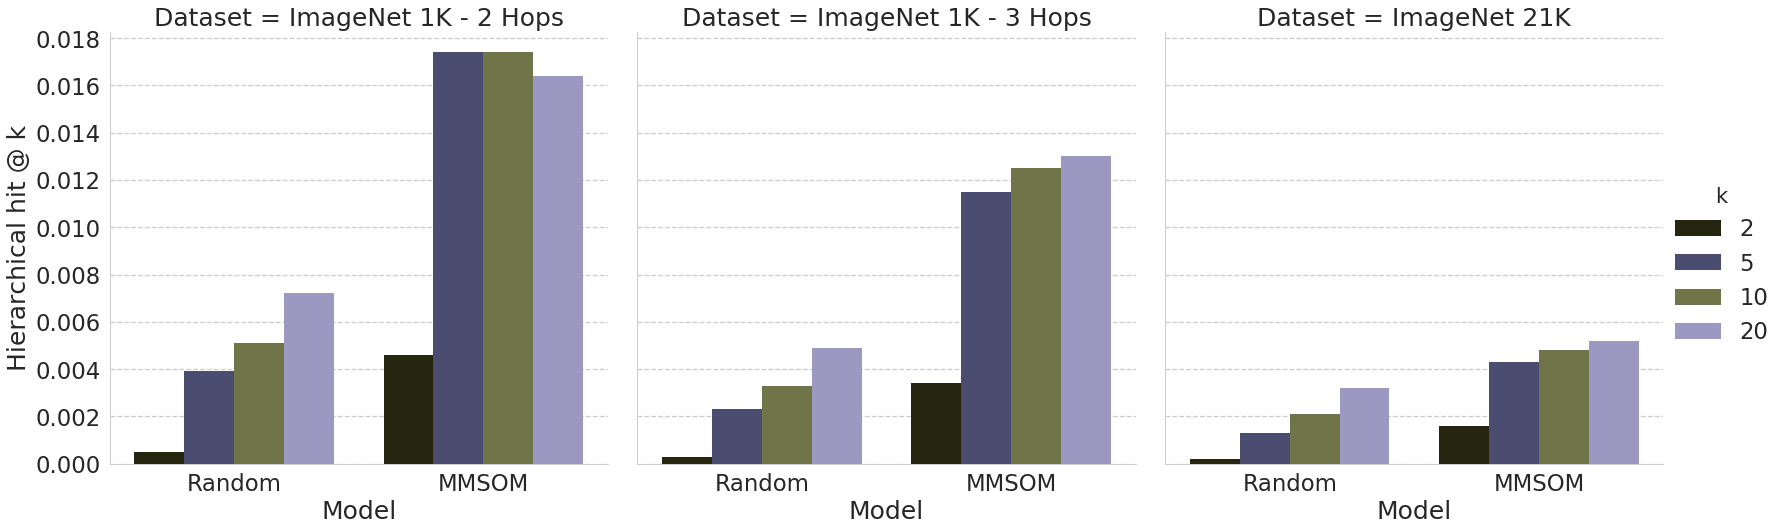
\includegraphics[width=\textwidth]{images/zero_shot_h_results.png}
    \caption{Zero-shot learning experiment - "hierarchical hit @ k" metric. The dip in performance on the \texttt{ImageNet1K - 2 Hops} dataset for the \texttt{MMSOM} model for $k=20$ w.r.t. $k=10$ and $k=5$ is due to the number of correct predictions growing slower than $k$. Before dividing by $k$, the mean number of predictions in the $CorrectSet$ were: $0.0909$, $0.1684$, $0.3244$ for $k=5$, $k=10$ and $k=20$, respectively.}
    \label{ZeroShotHierarchicalResults}
\end{figure}

\begin{table}[h]
    \centering
    \begin{footnotesize}
        \begin{tabularx}{\textwidth}{|X|c|c|c|c|c|}
            \hline
            \multirow{2}{*}{Dataset} & \multirow{2}{*}{Model}    & \multicolumn{4}{c|}{Hierarchical hit @ $k$}        \\
            \cline{3-6}              &                           & 2      & 5      & 10     & 20     \\ 
%            \hline
%            \hline
%            \multirow{2}{*}{ImageNet1K}          & Random        & 0.0031 & 0.0160 & 0.0254 & 0.0415 \\ 
%            \cline{2-6}                          & MMSOM         & 0.0171 & 0.0171 & 0.0158 & 0.0147 \\ 
            \hline
            \hline
            \multirow{2}{*}{ImageNet1K - 2 Hops} & Random        & 0.0005 & 0.0039 & 0.0051 & 0.0072 \\ 
            \cline{2-6}                          & MMSOM         & 0.0046 & 0.0174 & 0.0174 & 0.0164 \\ 
            \hline
            \hline
            \multirow{2}{*}{ImageNet1K - 3 Hops} & Random        & 0.0003 & 0.0023 & 0.0033 & 0.0049 \\ 
            \cline{2-6}                          & MMSOM         & 0.0034 & 0.0115 & 0.0125 & 0.0130 \\ 
            \hline
            \hline
            \multirow{2}{*}{ImageNet21K}         & Random        & 0.0002 & 0.0013 & 0.0021 & 0.0032 \\ 
            \cline{2-6}                          & MMSOM         & 0.0016 & 0.0043 & 0.0048 & 0.0052 \\ 
            \hline
        \end{tabularx}
    \end{footnotesize}
    \caption{Zero-shot learning experiment - "hierarchical hit @ k" metric.}
    \label{tab:ZeroShotHierarchicalResults}
\end{table}

\subsection{Analysis and interpretation of results}

Our approach out-performs the random classifier used as a baseline in all cases. This indicates that our model is indeed learning a meaningful representation of the data that goes beyond what it was originally trained to do, i.e. classification on 1000 class labels.

However, it is unclear to what extent our method is useful, given that the random classifier is one the weakest classifiers available.
An alternative baseline could have been to use the pre-trained AlexNet, but due to time constraints it was not feasible to include it in this work. It also bears mentioning that Frome et al. report better results across the board.

\end{document}

\end{document}